%; whizzy section -pdf xpdf -latex ./whizzypdfptex.sh
% latex beamer presentation.
% platex, latex-beamer でコンパイルすることを想定。 

%     Tokyo Debian Meeting resources
%     Copyright (C) 2007 Junichi Uekawa

%     This program is free software; you can redistribute it and/or modify
%     it under the terms of the GNU General Public License as published by
%     the Free Software Foundation; either version 2 of the License, or
%     (at your option) any later version.

%     This program is distributed in the hope that it will be useful,
%     but WITHOUT ANY WARRANTY; without even the implied warranty of
%     MERCHANTABILITY or FITNESS FOR A PARTICULAR PURPOSE.  See the
%     GNU General Public License for more details.

%     You should have received a copy of the GNU General Public License
%     along with this program; if not, write to the Free Software
%     Foundation, Inc., 51 Franklin St, Fifth Floor, Boston, MA  02110-1301 USA

% 実行順番
% sudo  ~/bin/usb-macbook-ir.c &
% real presentation (shell-command (concat "DISPLAY=:0.1 xpdf -fullscreen " (replace-regexp-in-string "tex$" "pdf"(buffer-file-name)) "&"))
% DISPLAY=:0.1 xpdf -fullscreen 

\documentclass[cjk,dvipdfmx,12pt]{beamer}
\usetheme{Tokyo}
\usepackage{ulem}
\usepackage{tabularx}

\usepackage{fancybox}
\usepackage{fancyvrb}   
\usepackage{float}

% commandline環境を定義。画面入出力についてはcommandline環境
% で表記する
\newenvironment{commandline}%
{\VerbatimEnvironment
  \begin{Sbox}\begin{minipage}{0.9\hsize}\begin{fontsize}{7.3}{7.3} \begin{BVerbatim}}%
{\end{BVerbatim}\end{fontsize}\end{minipage}\end{Sbox}
  \setlength{\fboxsep}{8pt}
% start on a new paragraph

\vspace{6pt}% skip before
\fcolorbox{dancerdarkblue}{dancerlightblue}{\TheSbox}

\vspace{6pt}% skip after
}
%end of commandline

\definecolor{dancerdarkblue}{rgb}{0,0.08,0.45}
\definecolor{dancernormalblue}{rgb}{0.8,0.9,0.95}
\definecolor{dancerlightblue}{rgb}{0.8,0.95,1}


%  preview (shell-command (concat "evince " (replace-regexp-in-string "tex$" "pdf"(buffer-file-name)) "&"))
%  presentation (shell-command (concat "xpdf -fullscreen " (replace-regexp-in-string "tex$" "pdf"(buffer-file-name)) "&"))

%http://www.naney.org/diki/dk/hyperref.html
%日本語EUC系環境の時
\AtBeginDvi{\special{pdf:tounicode EUC-UCS2}}
%シフトJIS系環境の時
%\AtBeginDvi{\special{pdf:tounicode 90ms-RKSJ-UCS2}}

\title{東京エリア Debian 勉強会}
\subtitle{資料}
\author{上川 純一 dancer@debian.org\\IRC nick: dancerj}
\date{2007年8月18日}
\logo{
\includegraphics[width=8cm]{image200607/openlogo-light.eps}}


% 間のタイトルページ用
\newcommand{\emtext}[1]{
\begin{frame}{}
 
\begin{minipage}{0.55\hsize}
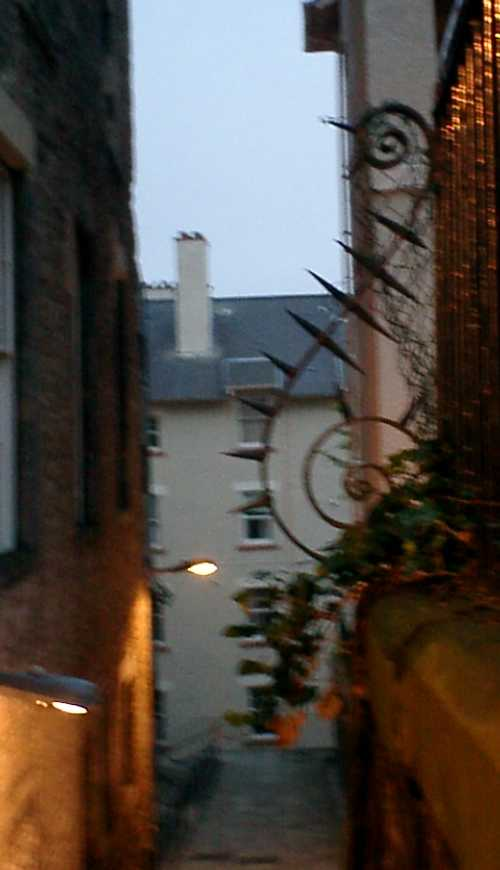
\includegraphics[width=1\hsize]{image200707/gurutitle.jpg}
\end{minipage}
\begin{minipage}{0.39\hsize}
 {\Huge #1
 }
\end{minipage}
\end{frame}
}

% 三択問題用
\newcounter{santakucounter}
\newcommand{\santaku}[5]{%
\addtocounter{santakucounter}{1}
\frame{\frametitle{問題\arabic{santakucounter}. #1}
%問題\arabic{santakucounter}. #1
\begin{minipage}[t]{0.8\hsize}
 \begin{itemize}
 \item
      \begin{minipage}{0.2\hsize}
      
\includegraphics[width=0.9\hsize]{image200703/janken-A.png}\end{minipage} 
       \begin{minipage}{0.6\hsize}
       A #2\end{minipage}\\
 \item
      \begin{minipage}{0.2\hsize}
      
\includegraphics[width=0.9\hsize]{image200703/janken-B.png}\end{minipage} 
       \begin{minipage}{0.6\hsize}
       B #3\end{minipage}\\
 \item
      \begin{minipage}{0.2\hsize}
      
\includegraphics[width=0.9\hsize]{image200703/janken-C.png}\end{minipage} 
       \begin{minipage}{0.6\hsize}
       C #4\end{minipage}\\
 \end{itemize}
\end{minipage}
}
\frame{\frametitle{問題\arabic{santakucounter}. #1}
%問題\arabic{santakucounter}. #1
\begin{minipage}[t]{0.8\hsize}
\begin{itemize}
 \item
      \begin{minipage}{0.2\hsize}
      
\includegraphics[width=0.9\hsize]{image200703/janken-A.png}\end{minipage} 
       \begin{minipage}{0.6\hsize}
       A #2\end{minipage}\\
 \item
      \begin{minipage}{0.2\hsize}
      
\includegraphics[width=0.9\hsize]{image200703/janken-B.png}\end{minipage} 
       \begin{minipage}{0.6\hsize}
       B #3\end{minipage}\\
 \item
      \begin{minipage}{0.2\hsize}
      
\includegraphics[width=0.9\hsize]{image200703/janken-C.png}\end{minipage} 
       \begin{minipage}{0.6\hsize}
       C #4\end{minipage}\\
\end{itemize}
\end{minipage}
\begin{minipage}[t]{0.15\hsize}
答えは:

\vspace{1cm}

  {\huge \hspace{1cm}#5}
  \hspace{-6cm}\includegraphics[width=4cm]{image200703/janken-#5.png}
 \end{minipage}}
}

\begin{document}
\frame{\titlepage{}}

\section{Intro}

\begin{frame}
 \frametitle{Agenda}
\begin{minipage}[t]{0.45\hsize}
  \begin{itemize}
  \item 注意事項
	\begin{itemize}
	 \item 飲食禁止
	 \item 政治/宗教/営利活動禁止
	\end{itemize}
  \item quiz
  \item 最近のDebian関連のイベント
	\begin{itemize}
	 \item 前回
	 \item OSC-Kansai
	\end{itemize}
 \end{itemize}
\end{minipage} 
\begin{minipage}[t]{0.45\hsize}
 \begin{itemize}
  \item cdn.debian.or.jp
  \item 最近はまったこと
 \end{itemize}
\end{minipage}
\end{frame}

\section{最近}

\begin{frame}
 \frametitle{前回のagenda}
\begin{minipage}[t]{0.45\hsize}
  \begin{itemize}
  \item 注意事項 
	\begin{itemize}
	 \item 飲食禁止
	 \item 政治/宗教/営利活動禁止
	\end{itemize}
  \item quiz
  \item Debconf7 報告
	\begin{itemize}
	 \item 概要
	 \item 議論
	\end{itemize}
 \end{itemize}
\end{minipage} 
\begin{minipage}[t]{0.45\hsize}
 \begin{itemize}
  \item Debconf workshop
	\begin{itemize}
	 \item 事前課題検討
	 \item Debconf で得るもの
	 \item Debconf を日本で開催するには
	\end{itemize}  
\item Debian 勉強会の今後の企画の検討
 \end{itemize}
\end{minipage}
\end{frame}

\section{DWN quiz}
\begin{frame}{Debian 常識クイズ}

Debian の常識、もちろん知ってますよね?
しらないとはずかしいけどしらないとは言えないいろいろなこと、
会長がこの目で確認しちゃうぞ!


今回の出題範囲は\url{http://www.debian.org/vote/2007/vote_003} にある投票
結果と、\url{http://lists.debian.org/debian-devel-announce/} にある最近の
アナウンス文書です。
\end{frame}

\subsection{問題}

\santaku{Debian Maintainers の提案は何をするものか}
{気に入らない Debian Developer を投票により追放する}
{Debian Developer より制限された権限をもつ Debian Maintainers を定義する}
{Debian Developer の品質を改善する}
{B}

\santaku{
Bits from the DPL: FTP assistants, DM, APT, sharing patches
で Sam Hocever が主張したのは
}
{パッチを共有しよう}
{もう会長としての仕事は終わった}
{Debian としては Ubuntu の殲滅が目標}
{A}

\santaku{
apt-get install の仕組みで大きな変化が発生したのは何か
}
{Suggests  をデフォルトでインストールするようになった}
{Recommends をデフォルトでインストールするようになった}
{Depends を無視するようになった}
{B}

\santaku{lenny のリリースゴールに入っているのはどれか}
{Debian の市場シェア40\% 以上の獲得}
{debian/rules が国際化対応}
{debian/changelog と debian/control は UTF-8}
{C}

\santaku{sparc32 になにがおきたか}
{次のリリースではサポートされなくなる}
{急にユーザが増えたので開発者を募集している}
{arm とバイナリ互換になった}
{B}

\section{最近の話題}

\emtext{Debian 勉強会}
\emtext{osc Kansai}

\section{cdn.debian.or.jp}
\emtext{事前課題の紹介}


\section{事前課題紹介}
\emtext{事前課題の紹介}
% pre work home work

\begin{frame}{事前課題問題}
「ここ最近 Debian を使っていて ハマったこと/ちょっと感激したこと」もしく
は「apt の sources.list はこう書く」
というタイトルで200-800文字程度の文章を書いてください。
\end{frame}

% (query-replace "\\subsection" "\\end{frame}\\begin{frame}")
% (query-replace "\\subsubsection" "\\textbf")

\begin{frame}{小室 文}

\textbf{ここ最近 Debian を使っていて ハマったこと/ちょっと感激したこと}

あんまりDebian特有ではないけど、Gimpってかなり使える事が判明して、結構感
動しました。元々MacでAdobe Photoshop/Illustratorを使っていたのですが、メ
インPCもDebianになったので、Gimpを使ってみようとあれこれしているうちに
Gimpってイイ!という事が判明。かなり使えるやつです。
後普通の人は知ってて当り前かもしれないけどgnome-utilsはなんかお得感一杯
(でもないけど)なパッケージでこういうのは結構小さな感動があったりします。

\end{frame}\begin{frame}{根岸 心}

\textbf{感動したこと}

開発環境を用意しようと、家に転がっていたPentiumIIのマシンにsargeをインストールしたのが、Debianとの出会いです。本番環境も当然Debianを使おうと思って、DELLのSC430を購入した後に、etchが登場したばかりで、安定的にSC430上で動作するDebianが無いことに気づき、仕方なくCentOSを利用することにしました。その時から、開発環境はDebian、本番環境(SC430)はCentOSで運用しています。CentOSマシンが増えてしまい、etchに全面移行することに踏み切れないため、CentOSをいじっている時間が長いですが、Debianマシンに戻る度に、あるべきところにあるべきファイルがある、通っているべきパスが通っていることに感動します。


\end{frame}\begin{frame}[containsverbatim]{Tsukasa Hamano}

\textbf{ここ最近 Debian を使っていて ハマったこと/ちょっと感激したこと}

最近自宅にオレオレaptレポジトリを作った事でお気に入りの環境が素早く構築
できるようになってちょこっと感動しました。

あと libdwarf-dev というライブラリのパッケージが sarge まであったのに
etch から無くなっていて悔しい思いをしたのですが、今日 libdw-dev という
同等のライブラリを見つけてマジで感激しました。

\textbf{apt の sources.list はこう書く}

\url{sources.list} はたくさん書くと update が遅くなって我慢できなくなるので

\begin{commandline}
 % m4 -DDIST=etch /etc/apt/sources.list.m4 > /etc/apt/sources.list
\end{commandline}

などと細かく分けた apt-line をその都度生成したり、symlink で切り替えた
りしていました。もっとカッコイイ方法があるんじゃないかと確信しています。

\end{frame}\begin{frame}{前田 耕平}

\textbf{ここ最近 Debian を使っていて ハマったこと/ちょっと感激し
   たこと}

テストではまって、家サーバをいまだにSargeからEtchに移行できていません。orz
久々に時間ができたので、Etchで構築したOpenBlocks266で、下記のように移行
しようと、Etchで環境作りました。

現状:Sarge\\
Apache 2.0 + mod\_php + PHP4 + PukiWiki + mod\_security 1.8

移行後の予定:Etch\\
Apache 2.2 + mod\_fcgid + PHP5 + PukiWiki + mod\_security 2.0

\end{frame}\begin{frame}{前田 耕平}

んで、phpinfo()はちゃんと結果を返すのに、PukiWikiでindex.phpにアクセスすると、failed
fopenでこけてしまうので、困ってしまったなぁと。
パッケージをそのまま使うのならaptitude update;aptitude
dist-upgradeでも良いのかもしれませんが、カスタマイズしている部分があるので、時間を割いて検証してみます。(いつだ?)
他のサーバもWebサーバが終わらないと検証できないので、Pending…。臆病者なので、いきなりアップグレードだなんてできません。w

ところで、PukiWikiってなぜパッケージないんでしょうね。別に必要はありませんけど。


\end{frame}\begin{frame}{前田 耕平}

他は、クライアントとしてSidを使っていてアップデートによって環境がおかしくなってしまっても、そのまま使っていたら結構馴れてしまうんだということに気がつきました。ダメ人間です。

\end{frame}\begin{frame}{前田 耕平}

\textbf{apt の sources.list はこう書く}

とくにないです。通常と違うのは、自宅のHobbit
monitorのサーバ&エージェントや、自宅鯖を運用するのに共通で使っているスクリプトを配布するのに、自宅のLANで立てているリポジトリを追加している程度です。

\end{frame}\begin{frame}[containsverbatim]{ARAKI Yasuhiro}

\textbf{apt の sources.list はこう書く}
\begin{commandline}
 deb http://cdn.debian.or.jp.nyud.net:8090/debian/ sid main
\end{commandline}

と書くことがたまにあります。\url{cdn.debian.or.jp}を他に変えても日本では速くないので
意味がありませんね。。
\end{frame}\begin{frame}[containsverbatim]{ARAKI Yasuhiro}
日本にいるときは

\begin{commandline}
 deb http://cdn.debian.or.jp/debian/ sid main
 deb-src http://cdn.debian.or.jp/debian/ sid main
\end{commandline}

ですね。etchまではjavaがなかったので行追加していましたが、現在は
変なツールをいれてないのでこれで十分です。

\end{frame}\begin{frame}{Hisashi MORITA}

\textbf{ここ最近 Debian を使っていて ハマったこと/ちょっと感激したこと}

久しぶりに新規インストールしたら、\url{/etc/default/locale}があるのに気が付か
ずはまりました。
また少し前ですが、teTeXからTeXLiveへ大きな問題なく移行できたのには感心し
ました。

\end{frame}\begin{frame}{Hisashi MORITA}

\textbf{apt の sources.list はこう書く}

うまく書けないのでbest practiceを知りたいところです。

\end{frame}\begin{frame}{山根秀樹}

\textbf{ここ最近Debian を使っていてハマったこと}

\begin{itemize}
 \item ハマったというか、シャットダウン時に必ず kernel log daemon が failed します。
 何故でしょう?
 \item 2.6.21 あたりから cpufreq なモジュールの読み込みに失敗します。なんか変更必要
 だったかな?
 \item util-linux でなんか含まれてないの (flock) があるぞ、というのをきんねこさんが書
 いていたので自前で修正してビルドしようとしたら、aclocal,automake,autoconf が入っ
 ている環境だとビルドにこけるという状態に陥った。何で誰も直してないんだ
       これ。
\end{itemize}
\end{frame}\begin{frame}{山根秀樹}
\begin{itemize}

 \item bcm43xx な無線LANカードを使っているのですが、2.6.18 までは問題なかったのに、そ
 れ以降(2.6.21、2.6.22など) が極度にスピードが遅くなった(タイムアウトもざら。ど
 うやら中身をまるっと書き換えてあるかららしいんですが、ドライバ側の対応待ちなのか
 なー?)
 \item tar のオプションを見ようとしたら、日本語の man になかった→LAMG=C で元の man を
 見ると新しい…でも GFDL のために Debian で新しく作ったものだった→infoを見てみる→
 日本語 info だとまともに表示されない orz
 \item ddtp で訳された description が apt で利用できるようになったのはいいのですが、
 内容が EUC-JP で書かれているために現在の UTF-8 な状態では文字化けしてまるで読め
 なかった。
\end{itemize}
\end{frame}\begin{frame}{山根秀樹}
\begin{itemize}
 \item onscripter で「ひぐらしのなく頃に」を遊ぼうとする→一部音声が再生されない orz
 \item anthy のアップデートで辞書ファイルの参照がおかしくて「☆」が入力できなかった
 (いや、「はて☆すた」とか書きたかっただけなんです)。
 \item あまりに普段 Debian だけで作業をしていて、家の Windows を起動しないでいたらパ
 スワードを思い出せなくなりました。
\end{itemize}

普通に使っているだけなのに日々ハマっていますね。うーむ。

\end{frame}\begin{frame}{山根秀樹}

\textbf{ちょっと感激したこと}

\begin{itemize}
 \item  E-mobile なカードを借りられたので設定をしてみたら、pppconfig で設定をさくさく
 できたこと。Windows よりある意味楽かも(PPP接続なんかも gnome のネットワーク設定
 からサクッとできるといいのかな。出来るかもしれないけど試してない)。岩松さんが
 Willcom の設定をしたときに接続設定の雛形があると良いかも、などといっていたが、こ
 れは E-mobile にもいえることかも。
\end{itemize}


\end{frame}\begin{frame}[containsverbatim]{山根秀樹}
\textbf{sources.list はこう書く}

nano ではなく vi で…じゃなくて、sources.list 自体には cdn.debian.or.jp だけ書い
ています。他のものについては、/etc/apt/sources.list.d/ 以下に用途に分けて書いて
ます。で、必要なくなったら(official に入った、配布を取りやめたなどの場合)コメ
ントアウトしたり消したりしています。

\begin{commandline}
deb http://www.debian-multimedia.org sid main
\end{commandline} 
ぐらいかなぁ、追加してるのは。

\end{frame}\begin{frame}[containsverbatim]{荒木 淳}

\textbf{apt の sources.list はこう書く}

使用 OS は、Debian etch stable です。
最初に参考文献の紹介です。以下のページを参考にしました。

\begin{itemize}
 \item   \url{http://www.debian.org/doc/manuals/apt-howto/ch-basico.ja.html}
 \item  \url{http://debian.fam.cx/index.php?install#content_1_37}
\end{itemize}

最適なミラーを探し出すのに、apt-spy と netselect-apt を使用しました。

\end{frame}\begin{frame}[containsverbatim]{荒木 淳}

最初に、apt-spy です。

\begin{commandline}

 $ sudo apt-spy update
 $ sudo apt-spy -d etch -s JP
\end{commandline}

これにより、以下の行が自動的に sources.list に書き込まれていました。既存の sources.list は
sources.list.bakに退避されました。

\begin{commandline}
 # sources.list generated by apt-spy v3.1
 deb http://ftp.jp.debian.org/debian/ etch main
 deb-src http://ftp.jp.debian.org/debian/ etch main
 #deb http://security.debian.org/ stable/updates main
\end{commandline}

\end{frame}\begin{frame}[containsverbatim]{荒木 淳}
 次に netselect-apt です。

\begin{commandline}
  $ sudo netselect-apt
\end{commandline}

これにより、以下の行が自動的に sources.list に書き込まれていました。既存の sources.list は
sources.list.orig に退避されました。

\begin{commandline}
 # the main Debian packages.
 deb http://ftp.dti.ad.jp/pub/Linux/debian/ stable main contrib
 # Uncomment the deb-src line if you want 'apt-get source'
 # to work with most packages.
 # deb-src http://ftp.dti.ad.jp/pub/Linux/debian/ stable main contrib
 # uncommenting the following line will enable security updates
 #deb http://security.debian.org/ stable/updates main contrib
\end{commandline}

\end{frame}\begin{frame}[containsverbatim]{荒木 淳}
上記に加えて、以下の行も推奨ということで追加しておきました。

\begin{commandline}
  deb http://cdn.debian.or.jp/debian etch main contrib non-free
 deb http://ftp.debian.or.jp/debian-security etch/updates main contrib
 non-free
 deb http://security.debian.org/ etch/updates main contrib non-free
\end{commandline}

\end{frame}\begin{frame}{Noriaki Sato}

\textbf{感動したこと}

初めて apt-get を使った時、すごく感動した(全然最近じゃない
けど、それ以外に debian で特別感動した事って無いような、、、

\section{}
\end{frame}\begin{frame}{Noriaki Sato}
\textbf{ハマったこと}

sarge → etch の upgrade で kacpid が暴走してハマった
のは5月に話したし、

samba を install した時、
Windows からマシンのアイコンは見えているのに、
「ネットワークパスが見つかりません」と出て繋げなくてハマった
のは CentOS の話だし、、、

そう言えば、この時、
CentOS のパッケージには cfdisk と w3m が見当たらなくて、
「やっぱり debian ってパッケージ多いんだなあ」
と改めて思いました(ちょっと感動)。

あと「ハマった」のとはちょっと違うけれど、
数ヶ月前、tDiary に脆弱性が見つかった時、
package がなかなか update されなかったので、
結局、package は uninstall して
自分で手動で入れ直したとゆー事がありました。

\end{frame}\begin{frame}{Noriaki Sato}
\textbf{おまけ}

debian はまった OR ハマった OR はまって OR ハマって に一致する日本語のペー
ジ 約 57,200 件中 1 - 50 件目 (0.19 秒) 

debian 感動 の検索結果 約 311,000 件中 1 - 50 件目 (0.20 秒) 

debian でハマった人に対して、感動した人は 5 倍程度いるようです。
めでたしめでたし。

#先月と同じネタですいません。

\end{frame}\begin{frame}{岩崎 修}

\textbf{ここ最近 Debian を使っていて ハマったこと/ちょっと感激したこと}

DELLのPowerEdge SC440にネットワークインストールのCDからインストールした
ところ、すっきりさっぱり、どこにもハマらずにインストール出来てしまったこ
とにちょっと感激しました。
後の様々な設定(webサーバやpostfix、などなど)もaptitudeのおかげで楽々イン
ストール。当たり前の用にwoodyの頃から使ってましたが、これは感激していい
ことなんだろうな、と思います。

\textbf{apt の sources.list はこう書く}

デフォルトのまま使っています。逆に、どのように書くのがスマートなのか、勉
強させていただきたいと思います。

\end{frame}\begin{frame}{山下 尊也}

第5回 関西 Debian 勉強会の時に、講師の方から頂いた資料に対して、
勉強会の表紙を作ろうと思い作ったのだが、pdfで配布資料と結合する
際にpdftkがインストールを試みると、libgcjの関係でインストール
出来なかった。時間がなかったので、依存関係の解決だけだったので、
snapshot.debian.netからパッケージを持ってきてインストールを
行ったが、やはり、このようなサービスが有志によって提供されている
って素晴らしいですね。

\end{frame}\begin{frame}{奥野 由紀}

\textbf{ここ最近 Debian を使っていて ハマったこと/ちょっと感激したこと}

実は今までDebianはちょっと敷居が高いな、と思っていました。
ですが、先日オープンソースカンファレンス.dbで
HPのサーバーが当たってしまったので、
思い切ってamd64版のetchを入れました。
(目録はGeekoのぬいぐるみだったのに……)
噂には聞いていましたが、Debian のパッケージは豊富ですね。
お題どおり「ちょっと感激」しました。
気がつけばsid + experimental にしてデスクトップPCとして常用しつつあります。
(サーバー用PCなのに……)

\end{frame}\begin{frame}{キタハラ}

\textbf{ここ最近 Debian を使っていて、ハマったこと/
   ちょっと感激したこと}

  これまで sarge でがんばっていたのですが、今回
のお題をみて、「これは etch を入れにゃーあかんな」
ということで入れてみました。

  sarge の時は、日本語入力の設定やサウンド出力で
苦労しましたが、etch ではあっさり使用できるように
なって、YouTube も クリック一発で Flash のプラグ
インが組み込まれ、あっさり動画が再生されました!
(おぉ、感動!)

  噂の GUI インストーラも試してみましたが、なか
なかよさげで、人に勧める時に良い感じ。(個人的には
動作がキビキビしている CUI で十分だが)

\end{frame}\begin{frame}{内山}

\textbf{ここ最近Debian を使っていてハマったこと/ちょっと感激したこと}

\begin{itemize}
 \item 玄箱でsarge $\rightarrow$ etch化があっけなく終わった事
 \item クロスdebootstrapで簡単にRFSが作成できてしまった事
\end{itemize}

\end{frame}\begin{frame}{小林儀匡}

\textbf{ここ最近 Debian を使っていて ハマったこと/ちょっと感激したこと}

aptによる依存関係の自動解決・ソフトウェアのコマンド一発インストール・ソースコードのコマンド一発取得が当たり前になりすぎて、
Debianを使っていても感激しないのですが、
他のOSを使っているとしょっちゅうDebianのすごさに感激します。
他のOSにはもう戻れません。

\end{frame}\begin{frame}{小林儀匡}

\textbf{apt の sources.list はこう書く}
昔は色々unofficialなパッケージのためのエントリを加えていましたが、
最近ではofficialなものだけで事足りるので (素晴らしい!!) 特に改変していません。
以前はtestingにはunstable経由でしかセキュリティサポートが入りませんでしたが、
最近では\texttt{security.debian.org}の\texttt{lenny/updates}経由でも入るようになったので、
それは取り込めるようにしています。

\end{frame}\begin{frame}[containsverbatim]{鈴木}

\textbf{ここ最近 Debian を使っていて ハマったこと/ちょっと感激し
   たこと}

Debianだからいいかな。

ハマる前の段階ですが、Debian GNU/Hurdのインストールができてません。
最初のインストールは出来て再起動後の設定がよく分からず、
ドキュメント読んでも進まず。MAKEDEVで何作ればいいの? fstabは?
使わないかも知れないけど、とりあえずインストールしてみたい。
いつの間にか楽なインストールや設定に慣れてしまった私。
勉強会までできるかどうか...

\textbf{apt の sources.list はこう書く}

普通のsources.listです。

\begin{commandline}
 deb http://ftp.riken.go.jp/pub/Linux/debian/debian/ unstable main
 contrib non-free
 deb-src http://ftp.riken.go.jp/pub/Linux/debian/debian/ unstable main
 contrib non-free
 deb http://www.debian-multimedia.org sid main
 deb-src http://www.debian-multimedia.org sid main
 deb http://ftp.debian-unofficial.org/debian sid main contrib non-free
 restricted
 deb-src http://ftp.debian-unofficial.org/debian sid main contrib
 non-free restricted
 ##deb http://www.mithril-linux.org/~henrich/debian/package/ ./
\end{commandline}

\end{frame}\begin{frame}{David Smith}


\textbf{ここ最近 Debian を使っていて ハマったこと/ちょっと感激したこと}
仕事で設定ファイルをパッケージにまとめたかったなと思ってやってみたら
cdbsで意外に簡単で感動しました。以前cdbs等のツールについてお話しが
あったと思いますが誰でもできることはあまり示されなかったかもしれないので、
こんなような作ったと紹介したいです。

\end{frame}\begin{frame}[containsverbatim]{David Smith}

\textbf{"/"ファイルシステムのようなディレクトリ階層を作成。}
設定ファイルをそこで管理する。例えば~/project/shorewall-basic-settingsだったら
そこにetc/shorewallディレクトリを作って設定ファイルを格納。
僕のプロジェクトは以下の感じ、

\begin{commandline}

 $ find ~/project/shorewall-basic-settings
 .
 ./etc
 ./etc/shorewall
 ./etc/shorewall/interfaces
 ./etc/shorewall/policy
 ./etc/shorewall/rules
 ./etc/shorewall/zones
 ./etc/default/shorewall
\end{commandline}

\end{frame}\begin{frame}[containsverbatim]{David Smith}

\textbf{そのディレクトリにdebianディレクトリを作成、以下のファイルを記入}
\begin{commandline}
==./debian/rules==
#!/usr/bin/make -f
DH_ALWAYS_EXCLUDE".svn"
include /usr/share/cdbs/1/rules/debhelper.mk

==./debian/install==
etc/shorewall/*
etc/default/shorewall

==./debian/changelog==
dds-shorewall-basic-settings (1.0) unstable; urgency=low

 * Initial release of shorewall settings package.

-- David Smith <davidsmith@acm.org>  Thu, 16 Aug 2007 14:12:45 +0900

==./debian/control==
Source: dds-shorewall-basic-settings
Section: misc
Priority: extra
Build-Depends: debhelper (>= 5), cdbs
Maintainer: David Smith <davidsmith@acm.org>
Standards-Version: 3.7.2

Package: dds-shorewall-basic-settings
Architecture: all
Depends: shorewall, ${misc:Depends}
Description: Customized basic shorewall configuration for my servers
These settings set up shorewall to run allowing basic services that all
hosts should support. It blocks everything except ping, ssh, and UDP
traceroute from the outside world.

==./debian/copyright==
Copyright 2007 David Smith <davidsmith@acm.org>. Public Domain.
\end{commandline}

\end{frame}\begin{frame}{David Smith}

\textbf{終わりに}

debianディレクトリはchangelog以外ほとんど変更しないので管理しやすくて
明瞭だと思います。

\textbf{apt の sources.list はこう書く}
最近sources.listを空っぽにしてsources.list.dにstable.list、testing.list、
security.listなどで分別してみました。目的としてはcron-aptでsecurity.list
だけに指したり自作パッケージで専用レポジトリを追加削除したりしたかったの
ですが、結局libaptのバグらしくてsources.list.dを使っているならDir::Etc::SourcesList
を設定しても効かないみたいだったから止めてしまって新規インストールのような
綺麗にまとまったsources.listを書くことにしちゃいました。

\end{frame}\begin{frame}{碇}

Debianはもっぱらサーバーとして利用しています。
メールサーバー兼webサーバーが一台、開発ようのサーバーを2台動作させていま
す。現在PHPによるサービスを開発していまして、その際の設定で躓いたことを
報告します。

開発自体はWindowsで行っていまして、IDEとしてPDTというZendが提供している
eclipseプラグインを使用しています。サーバーへのデプロイとブレークポイン
トを設定してのデバッグができるのですが、軽くはまっときました。
デプロイ自体はsamba経由で設定できたのですが、デバッグがなかなかうまくで
きませんでした。
\end{frame}\begin{frame}[containsverbatim]{碇}

ZendDebuggerをphp.iniに設定するさいにWindowsとLinuxで書式が違うことに
気がつかずはまりました。

\begin{itemize}
 \item Windows:
\begin{commandline}
zend_extension_ts="c:\php\ZendDebugger.so"
\end{commandline} 
\item Linux:
\begin{commandline}
zend_extension="/usr/local/lib/ZendDebugger.so"
\end{commandline}
\end{itemize}

上記のように設定しなければいけない所をDebianでWindowsの設定をしていたた
め動作しなかったのでした。

\end{frame}


\section{上川}

\begin{frame}{Debian GNU/kFreeBSD}

 最近はまったこと。

\begin{itemize}

 \item apt-listbugs がどうも Debian GNU/kFreeBSD と GNU/Hurd で動かない
らしい。

 \item xorg で xrandr 
 \item tex4ht
\end{itemize} 

\end{frame}


\newcommand{\graphicspage}[1]
{
\begin{frame}{}
 \includegraphics[width=\hsize]{#1}
\end{frame}
}

\graphicspage{image200708/kfreebsd-install-0.png}
\graphicspage{image200708/kfreebsd-install-1.png}
\graphicspage{image200708/kfreebsd-install-2.png}
\graphicspage{image200708/kfreebsd-install-3.png}
\graphicspage{image200708/kfreebsd-install-4.png}
\graphicspage{image200708/kfreebsd-install-5.png}


\section{サマリー}

\begin{frame}{サマリー}

\begin{tabularx}{\hsize}{|l|X|X|}
\hline
 & 要素 & 例 \\
\hline
\hline
\end{tabularx}
\end{frame}

\section{最近のイベント}
\begin{frame}{最近のイベント}
\begin{itemize}
 \item 8月25日 Install Festa, BSP
 \item 9月15日 Debian勉強会
 \item 10月5-6日 OSC Tokyo/Fall
 \item 10月20日 Debian勉強会
\end{itemize}
\end{frame}

\end{document}
